\documentclass[a4paper,
               %boxit,        % check whether paper is inside correct margins
               %titlepage,    % separate title page
               %refpage       % separate references
               %biblatex,     % biblatex is used
               keeplastbox,   % flushend option: not to un-indent last line in References
               %nospread,     % flushend option: do not fill with whitespace to balance columns
               %hyphens,      % allow \url to hyphenate at "-" (hyphens)
               %xetex,        % use XeLaTeX to process the file
               %luatex,       % use LuaLaTeX to process the file
               ]{jacow}

\usepackage{pdfpages,multirow,ragged2e} %
%\usepackage[inkscapelatex=false]{svg}

\makeatletter%
	\ifboolexpr{bool{xetex}}
	 {\renewcommand{\Gin@extensions}{.pdf,%
	                    .png,.jpg,.bmp,.pict,.tif,.psd,.mac,.sga,.tga,.gif,%
	                    .eps,.ps,%
	                    }}{}
\makeatother

\ifboolexpr{bool{xetex} or bool{luatex}} % test for XeTeX/LuaTeX
 {}                                      % input encoding is utf8 by default
 {\usepackage[utf8]{inputenc}}           % switch to utf8

\usepackage[USenglish]{babel}

\begin{document}

\title{Head-Tail Mode Zero Instability Growth Rate \\ Studies 
In The CERN SPS}

\author{E. de la Fuente\thanks{elena.de.la.fuente.garcia@cern.ch}, I. Mases\thanks{ingrid.mases.sole@cern.ch}, H. Bartosik, C. Zannini \\ CERN, Geneva, Switzerland} 

\maketitle

%
\begin{abstract}
The Head-Tail mode 0 instability growth rate is related to the real part of the transverse beam coupling impedance. The SPS transverse impedance model, which includes the major impedance contributions in the machine, can be benchmarked through measurements of growth rate as function of chromaticity. This paper summarizes the new methodology established to explore a wider range of chromatic frequency shift, and presents the measurements performed after the LHC Injectors Upgrade (LIU) for two sets of machine optics: nominal low gamma transition optics (Q20) and the former standard (Q26) optics. The measurements are compared with the current impedance model to further study its degree of accuracy.   
\end{abstract}


\section{INTRODUCTION}
The SPS transverse impedance model contains the contribution of the vast majority of accelerator components in the machine \cite{salvant:ipac19-weypls1}. The transverse impedance of these devices can be computed through analytical models, Wakefield simulations and/or bench measurements\cite{Zannini:2013wjh}. The current impedance model is used in particle tracking simulations \cite{MounetDelphi, OeftigerPyHEADTAIL} in order to predict beam stability. The computed impedance model needs to be benchmarked through beam-based measurements of related properties, such as coherent tune shift vs. intensity~\cite{rumolo:tuneshift}, TMCI thresholds~\cite{Bartosik:2014ria}, and Head-tail growth rates vs. chromaticity; the latter being the subject of study of this paper.

The CERN SPS operates above transition energy, thus the head-tail mode 0 is unstable for negative chromaticity, $\xi=Q/Q'$, that is, negative chromatic frequency shift, $f_{\xi} = \xi Q f_\textrm{rev} / \eta$. The instability growth rate $\tau^{-1}$ depends on the real part of the effective driving impedance $Z^\textrm{eff}_{\perp, \textrm{dip}}$ by~\cite{Chao:book}:

\begin{equation}\label{eq1}
    \tau^{-1}(\xi) = \pi^{-\frac{3}{2}} \frac{  Re \left [ Z^\textrm{eff}_{\perp, \textrm{dip}}(\xi) \right ] N r_0 c^2 }{8\pi^2 \gamma Q_{\perp} \sigma_z},
\end{equation}
where $N$ is the number of protons per bunch, $r_0$ is the electron radius, $c$ is the speed of light, $\gamma$ is the relativistic factor, $Q_{\perp}$ is the transverse tune and $\sigma_z$ is the RMS bunch length. 
Consequently, analyzing the behavior of the instability growth rates as function of the chromatic frequency shift can provide valuable insights into the impedance spectrum. Previous characterization of Head-tail mode zero growth rates were reported in Ref.~\cite{Zannini:2015eqc}. These measurements were performed pre-LS2 for two sets of optics: low-gamma transition Q20 \cite{HannesOpticsQ20} and the former nominal Q26 optics.

In the framework of the LHC Injectors Upgrade (LIU), a further benchmark of the present impedance model was required. The measurements presented in this paper were carried out on a broader chromatic range compared to pre-LIU measurements. For this, we profited from the Q26 optics' smaller slip factor $\eta = 1/\gamma_t ^2 - 1/\gamma^2$ that defines the conversion from chromaticity to chromatic frequency $f_{\xi}$. 
Using the new chromaticity trim procedure explained in this paper, the SPS impedance model can be benchmarked up to higher frequencies. The two different approaches in the way of changing the chromaticity along the cycle are explained in the following section.

\section{METHODOLOGY}
The measurements were performed with a single-bunch beam with low intensity, varying from $1\cdot 10^{10}$ to $3\cdot 10^{10}$ protons per bunch (p/b). For each set of optics, the tunes were set to the nominal operation values, measured and adjusted with the newly developed Laslett correction application~\cite{MasesSole:2022wlr}. Beam quality was improved by turning the Landau RF system ON  \cite{doubleRF:2019} and setting the octupole strength (LOF and LOD) to zero. Throughout all the measurements, the transverse feedback was turned OFF, only to be turned ON for the damper studies that are detailed in the dedicated subsection. 

\begin{figure}[!htb]
   \centering
   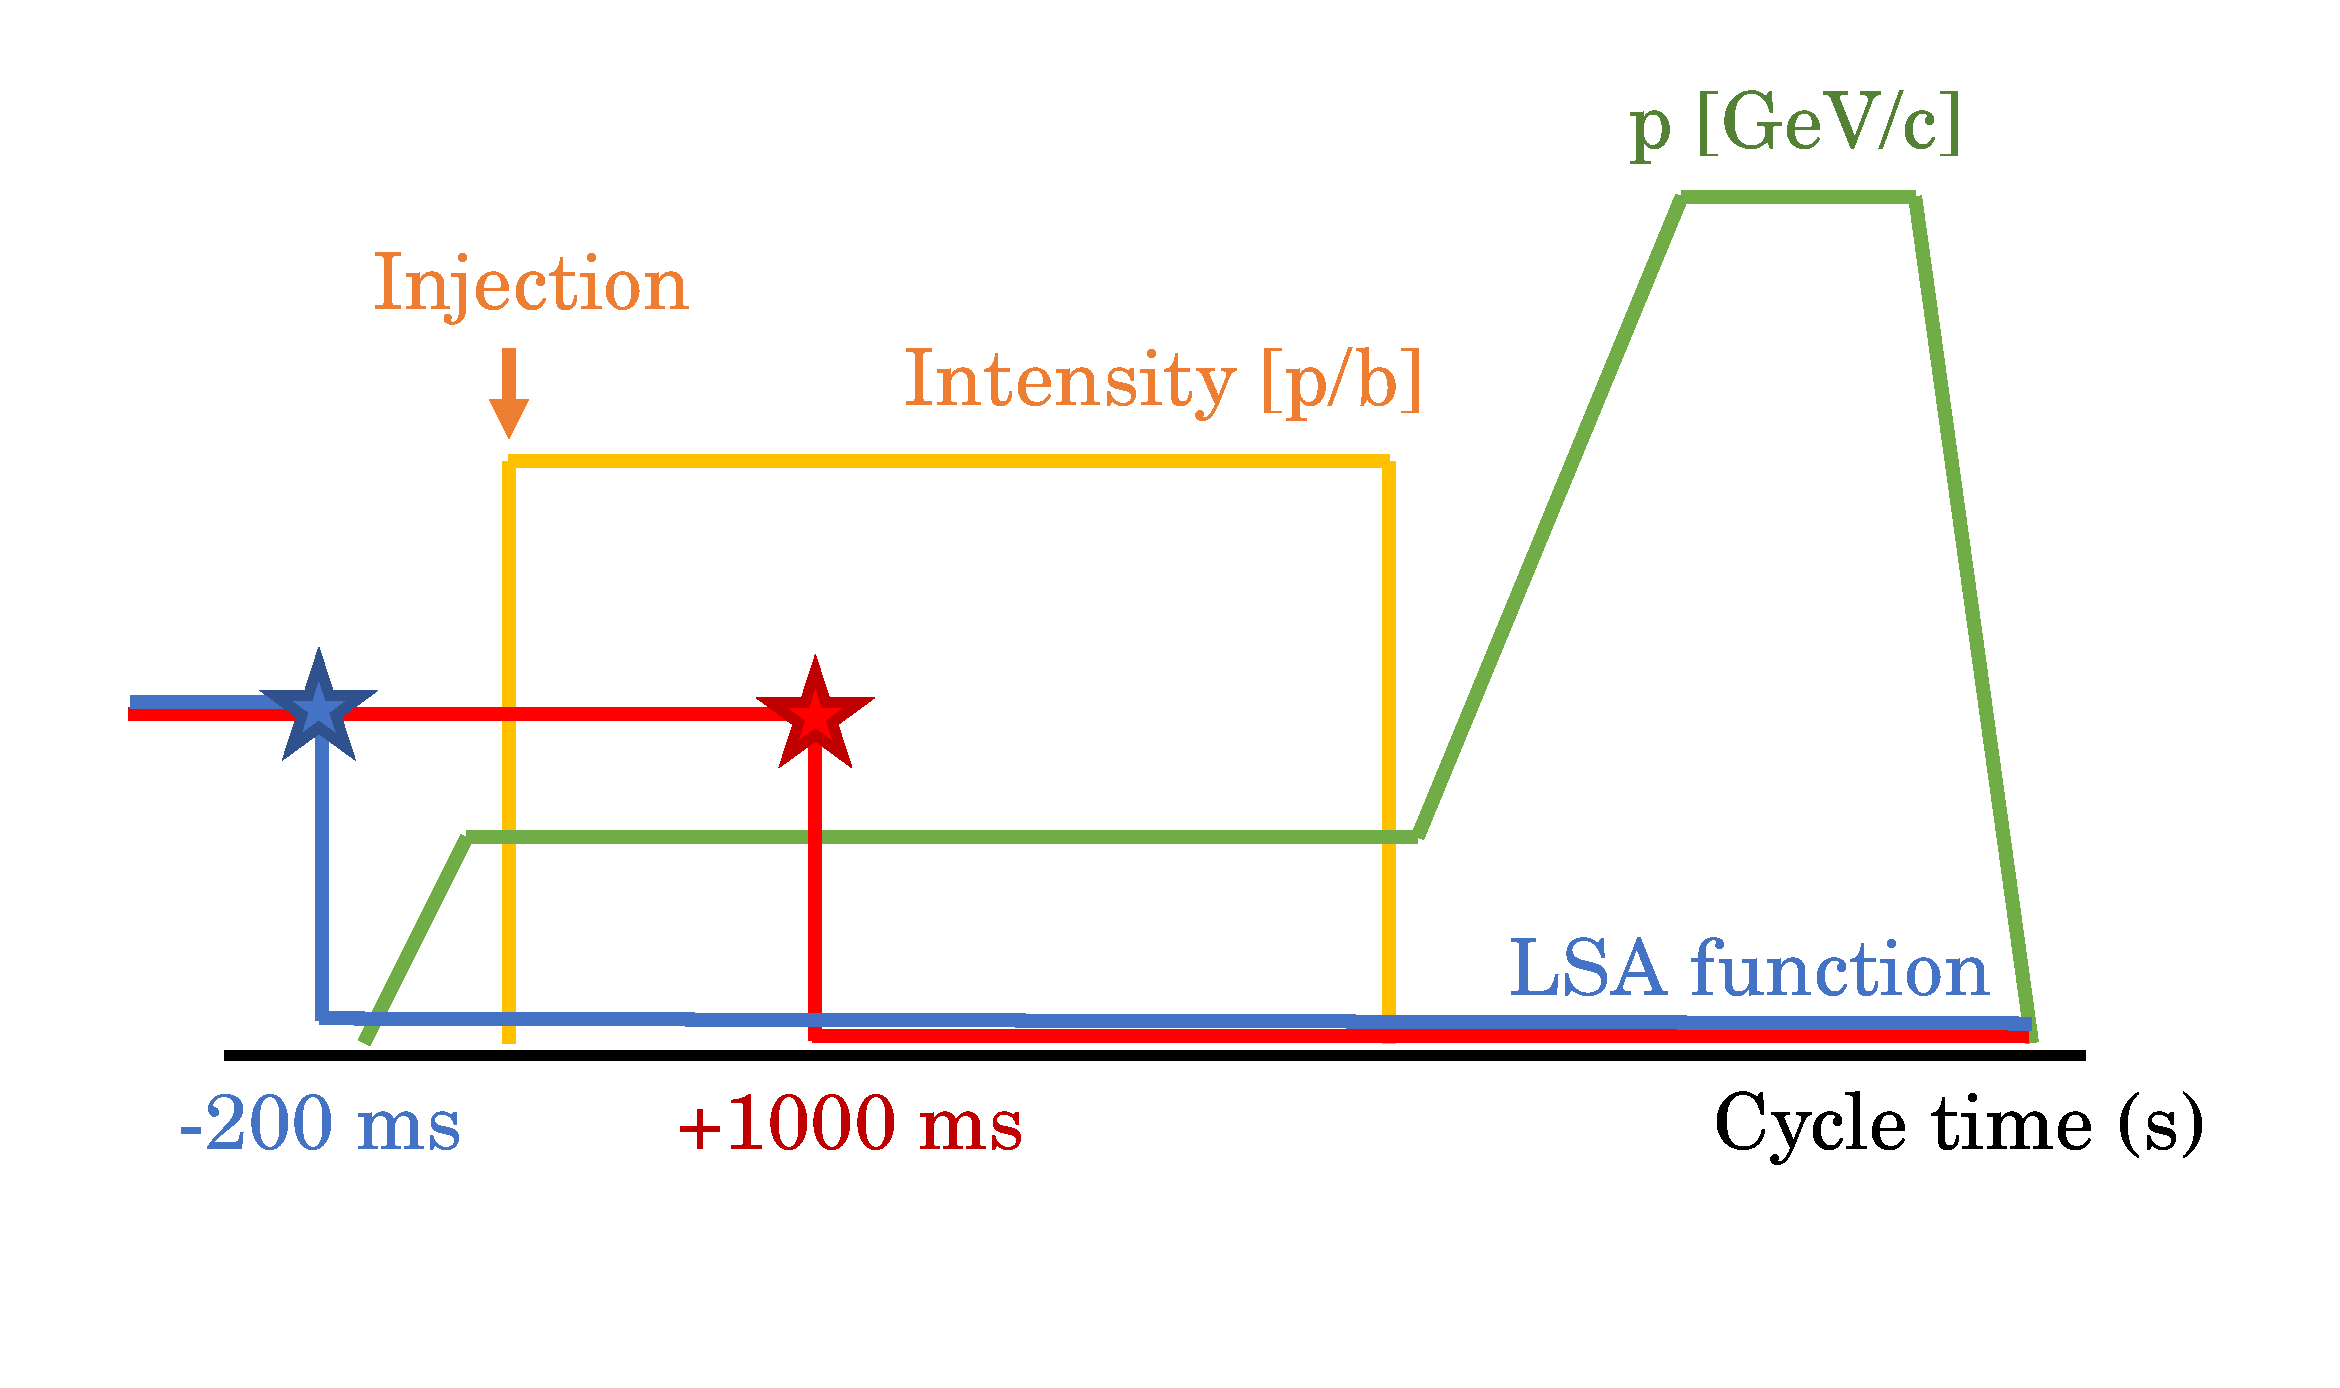
\includegraphics[width=\columnwidth]{img/WEPL155_f1.pdf}
   \caption{Conceptual schematic of the vertical chromaticity trim strategy versus cycle time. In blue, the former trim function, with the step before injection. In red, the trim function tested during these measurements. In yellow, the beam intensity (for a stable beam case), and in green, the momentum, were added for illustrative purposes.}
   \label{fig:trim}
\end{figure}

Chromaticity was changed using the LSA application \cite{Arduini:2012hma}, by changing the value function of the \texttt{QPV} knob. To trigger the instability, one has to find the knob value that makes $\xi$ < 0. The offset between the knob and the actual chromaticity of the machine was characterized during these measurements, obtaining a value of $\xi_{y, \text{knob}} - \xi_{y, \text{SPS}} = 0.12$ for Q26 and $0.10$ for Q20. This chromaticity calibration study was presented in Ref.~\cite{delafuente2023measurements}, where a dependency with the supercycle configuration was also observed.
\begin{table}[!hbt]
   \centering
   \caption{PyHEADTAIL simulation parameters for Q20 and Q26 optics.}
   \begin{tabular}{p{37mm} c c}
       \toprule
       \textbf{Variable, symbol} & \textbf{value Q20} & \textbf{value Q26}  \\               
       \midrule
           Betatron tunes, $Q_x/Q_y$  &  20.13/20.18 & 26.13/26.18   \\ %[3pt]
           Gamma at transition, $\gamma_t$  & 18 & 22.8   \\ %[3pt]
           Average beta function, \\ $\bar{\beta_{x,y}}$ [m] & 54.6 & 42 \\ %[3pt]
           $2^{nd}$ order chromaticity, \\ $Q''_x/Q''_y$ [$10^2$]  & 2.7/6.6 & 5/1.3  \\ %[3pt]
           $3^{rd}$ order chromaticity, \\ $Q'''_x/Q'''_y$ [$10^5$]  & -18.7/14.5 & -4/2  \\ %[3pt]
           Number of bunch \\ slices/macro-particles  & 70/$3\cdot10^5$ & 70/$3\cdot10^5$  \\ %[3pt]
       \bottomrule
   \end{tabular}
   \label{t1}
\end{table}


When chromaticity is below zero, the beam becomes unstable, showing sharp intensity losses in the Beam Current Transformer (BCT) monitor display. The expected exponential growth of the beam average centroid position can be observed when looking at the vertical acquisitios of the Qmeter application. To obtain the growth rate from the centroid turn-by-turn positions, the Moving Window Fourier Transform (MWFT) was used, as described in Ref.~\cite{burkhardt2002coherent}. The parameters of the MWFT have to be chosen wisely since they have an impact on the accuracy of the estimated growth rate, and should be kept constant for all the analysed datasets \cite{delafuente2023simulations}.

A refined chromaticity scan was performed. Since in these studies we were only interested in the vertical plane, the horizontal chromaticity $\xi_x$ was kept positive and constant for all the vertical chromaticity scan. For knob chromaticity values $0 > \xi_{y, \text{knob}} > -0.6 $ the chromaticity trim was made before injection of the beam in the SPS (see blue curve in Fig.~\ref{fig:trim}) and the instability started some milliseconds after injection. On the other hand, for knob values $-0.6 \geq \xi_{y, \text{knob}} \geq -1.3$, if the trim was kept before injection, the beam became unstable already at injection, therefore the exponential growth of the vertical signal could not be observed due to losses. To overcome this problem and to be able to measure the growth rate at chromaticity knob values $\xi_{y, \text{knob}} \leq -0.6$, the best strategy to follow is to apply the trim 1000 ms after injection (see red curve in Fig.~\ref{fig:trim}). This way, the beam is stable at injection and it becomes unstable when the chromaticity trim is done.


\subsection{Transverse Feedback Studies}

Following the strategy described in the previous section, every time a chromaticity trim is done, the currents of the sextupole magnets take around 60 ms to reach the new value, thus, a 10 ms step-like transition in chromaticity is not feasible.
During the measurements, it was observed that, in some cases, the instability appeared before the sextupole currents had reached the target value. Because of this phenomenon, there is an uncertainty in the chromaticity at which the instability was triggered \cite{delafuente2023measurements}.

An attempt was made to address this issue using the SPS transverse damper which is a feedback system that measures the bunch-by-bunch oscillations and damps them by means of fast electrostatic kickers. The new strategy consisted in doing the chromaticity trim before injection and inject the beam with the damper ON. This way, the head-tail mode 0 instability is suppressed by the damper, the beam is stable at injection and the sextupole currents reach the desired target value before injection. Then, the damper is switched OFF some milliseconds after injection, and the instability occurs. 

\begin{figure}[!htb]
   \centering
   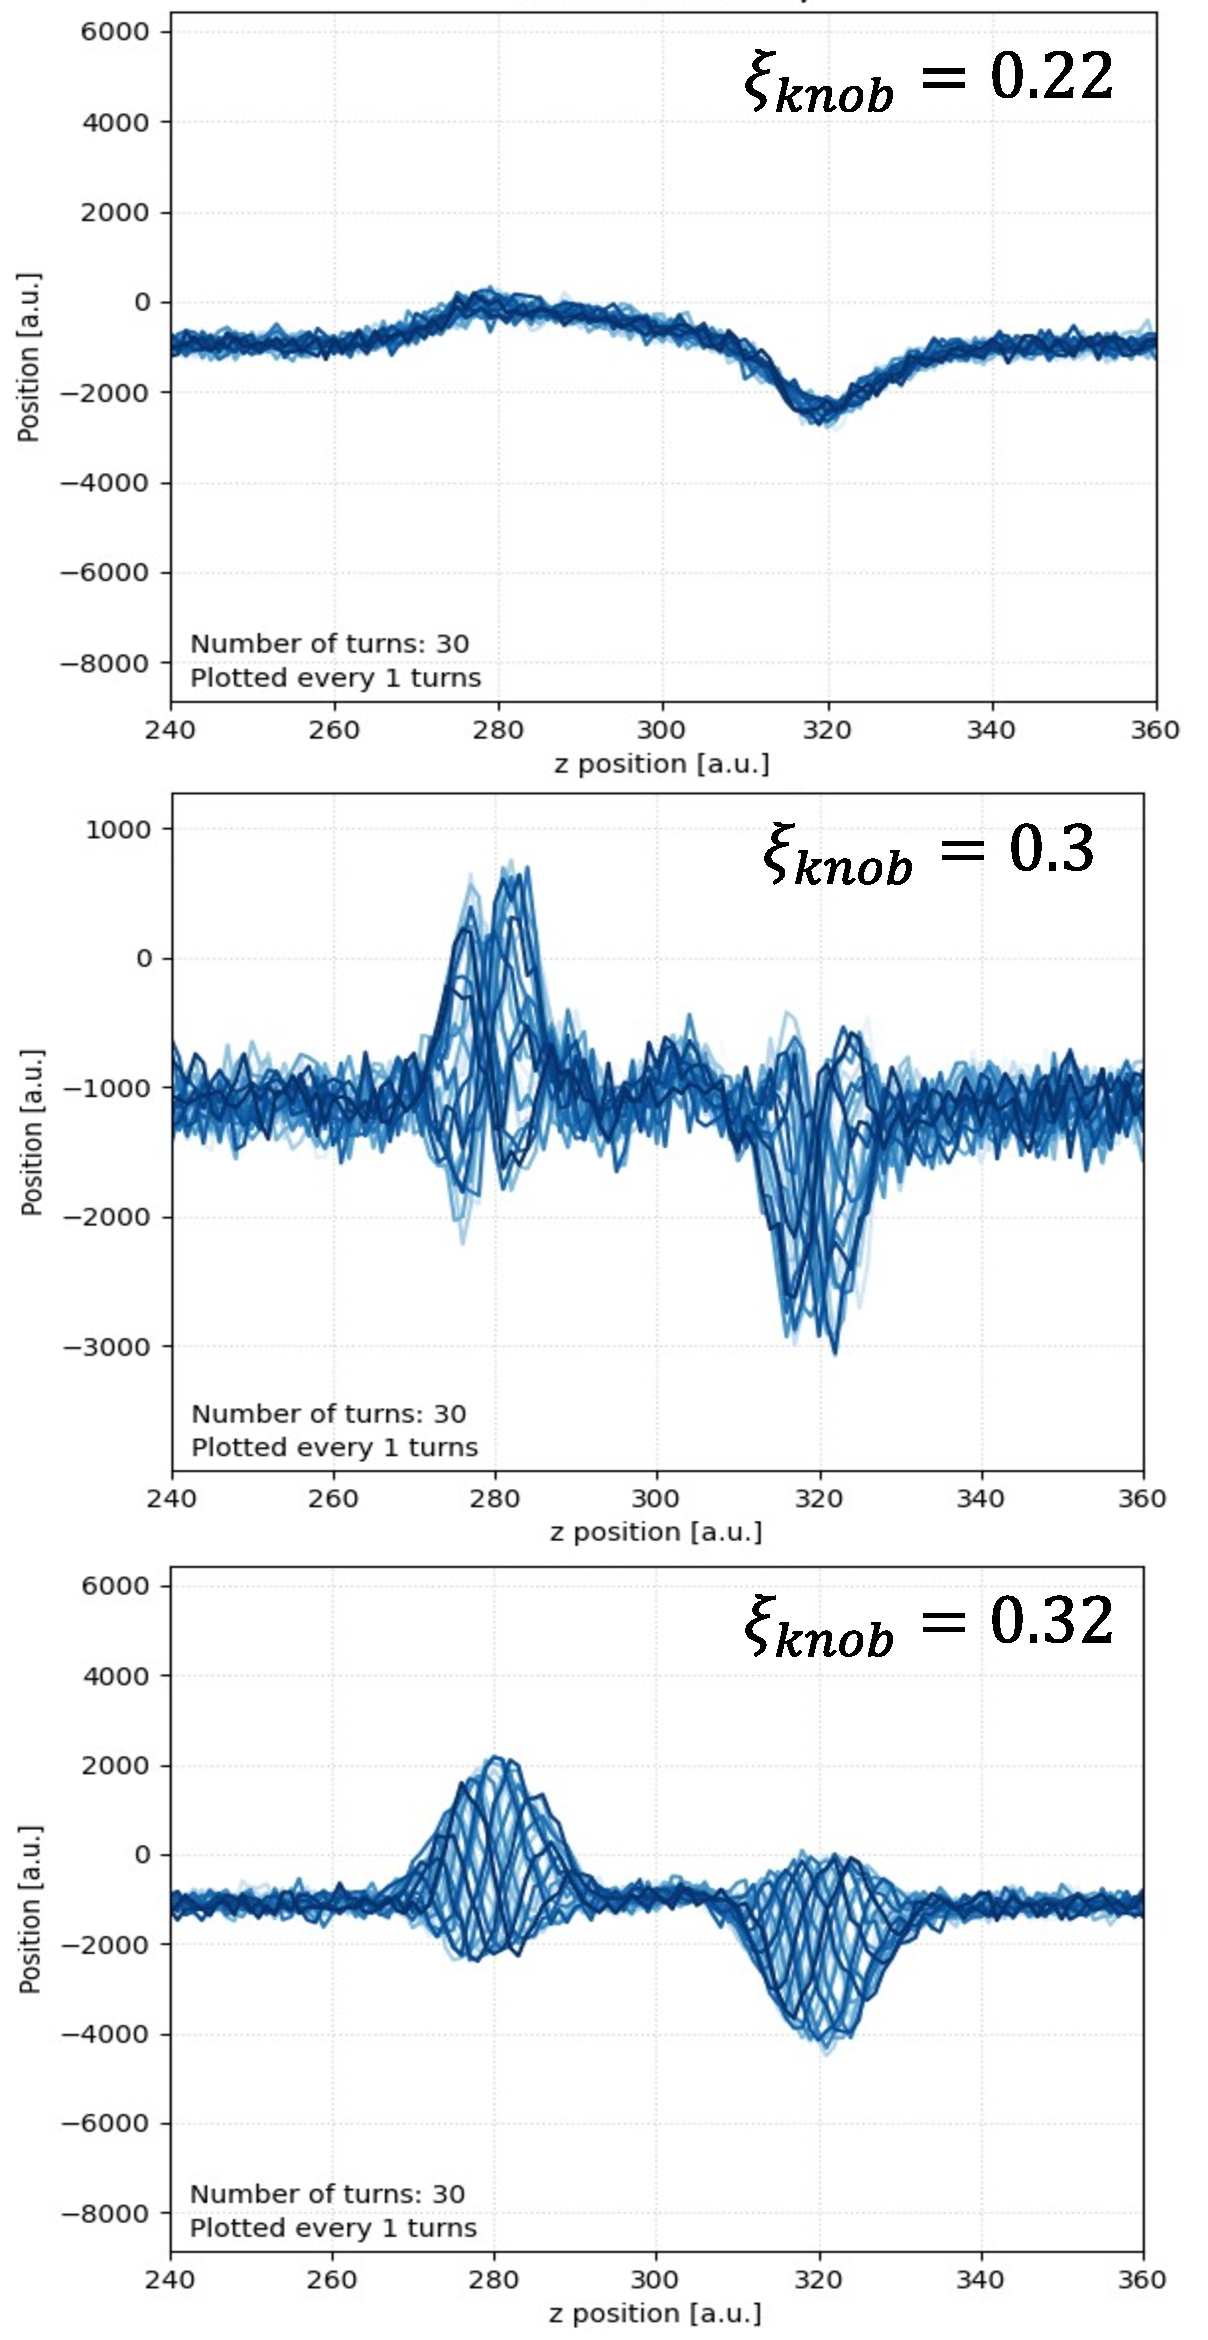
\includegraphics[width=.8\columnwidth]{img/WEPL155_f2.pdf}
   \caption{Vertical intrabunch motion captured with the Head-Tail monitor application for different chromaticity knobs, with the transverse feedback damper ON.}
   \label{fig:intrabunch}
\end{figure}

Using this approach, the uncertainty in chromaticity is avoided because the instability starts when the sextupoles currents have completely changed. This new method was tried during measurements and it was found that the actual transverse damper can only stabilize the beam with $\xi_{y, \text{knob}} \geq -0.22$. As seen in Fig.~\ref{fig:intrabunch} the intrabunch motion of the beam was monitored using the Head-Tail Monitor application, showing that it is not possible to implement the new strategy for $\xi_{y, \text{knob}} < -0.22$. After these observations, the possibility of using the wide-band feedback system in the SPS was proposed, in order to stabilize the beam for $\xi_{y, \text{knob}} < -0.22$. 

\section{SIMULATIONS}
Growth rates of the instability have been simulated for different chromaticities with the PyHEADTAIL macroparticle tracking code \cite{OeftigerPyHEADTAIL} using the most recent SPS impedance model obtained from \cite{{impedance-web},{CZ:SPSmodels}} for the two sets of optics. The
simulations and growth rate analysis have been carried out under the same conditions as the measurements described above, keeping the same MWFT settings. The relevant parameters used in the simulations are summarized in Table ~\ref{t1} for Q20 optics and Q26 optics. All the values are based on Table 4.6 from \cite{Bartosik:1644761}. 

A bi-dimensional convergence study was carried out in order to select the number of slices and number of macro-particles to use in the simulations. As presented in Ref.~\cite{delafuente2023simulations}, the number of slices to ensure convergence should be no less than 60. The number of macro-particles did not have a strong impact on the growth rate but does affect the computational cost of the simulations.

\section{RESULTS}

Results for Q20 measurements and simulations are shown in Fig.~\ref{fig:q20}. The vertical error bar accounts for the bunch population standard deviation of the measurements combined with the growth rate fit error from the analysis. For the range of chromatic frequency analysed for Q20, simulations and measurements show outstanding agreement.
\begin{figure}[!htb]
   \centering
   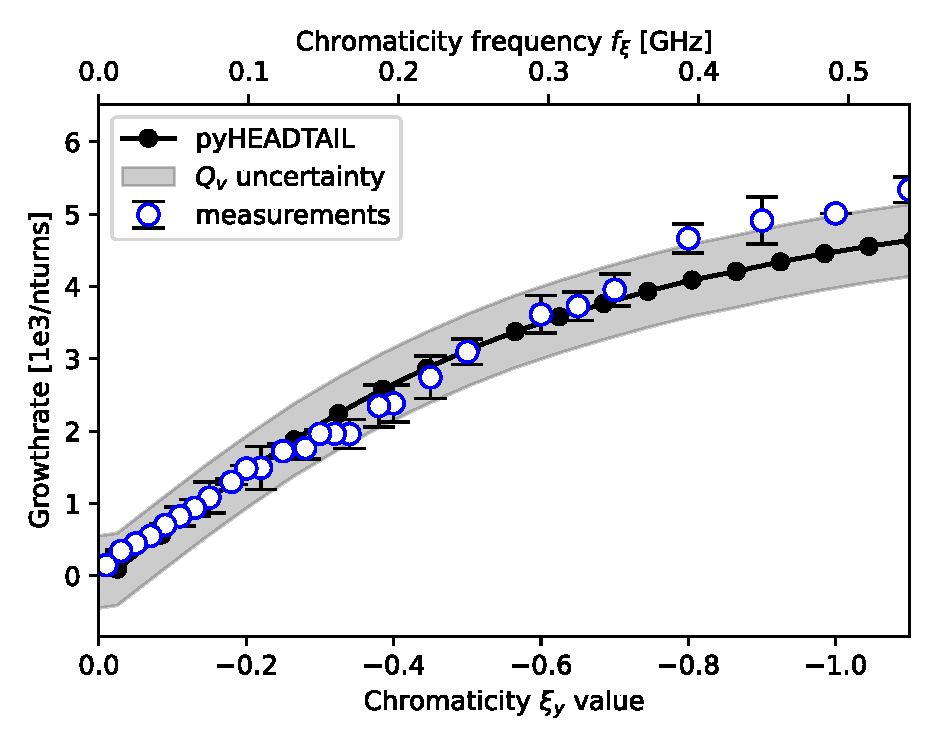
\includegraphics[width=1.0\columnwidth]{img/WEPL155_f3.pdf}
   \caption{Measurements and PyHEADTAIL simulations results for Q20 optics versus chromaticity $\xi$ and chromatic frequency $f_{\xi}$. The shaded area corresponds to the uncertainty of non-linear chromaticity values used in the simulations.}
   \label{fig:q20}
\end{figure}

\begin{figure}[!htb]
   \centering
   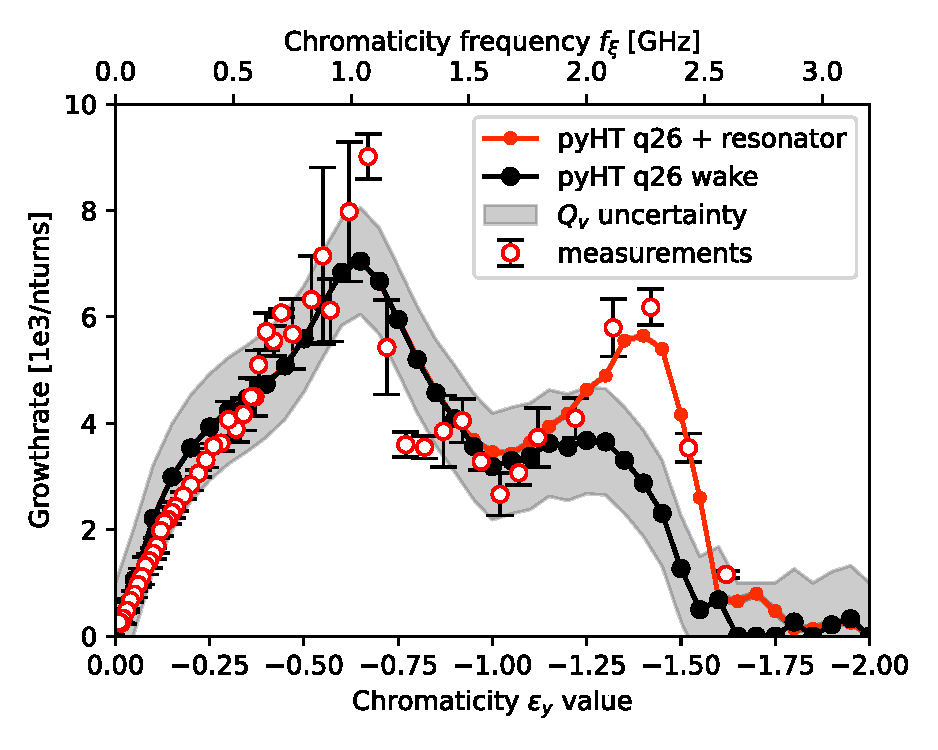
\includegraphics[width=1.0\columnwidth]{img/WEPL155_f4.pdf}
   \caption{Measurements and PyHEADTAIL simulations results for Q26 optics versus chromaticity $\xi$ and chromatic frequency $f_{\xi}$. The shaded area corresponds to the non-linear chromaticity uncertainty. The line in red uses the effective impedance model with an added resonator.}
   \label{fig:q26}
\end{figure}

Covering a wider range of chromatic frequency, results for Q26 measurements and simulations are shown in Fig.~\ref{fig:q26}. We found good agreement for lower and mid frequencies. However, around 1.0 GHz the instability turned very fast and difficult to measure and analyse, hence the larger error bars. The biggest discrepancy is found after 2.0 GHz, where an unexpected second peak is observed in the measurements. 

In order to understand the origin of this peak around 2.4 GHz, a non-linear chromaticity study was performed, varying both $Q''_y$ and $Q'''_y$ values in logarithmic steps. It was found that increasing the second-order chromaticity decreases the growth rate amplitude, whilst increasing the third-order chromaticity shifts the growth rate curve to higher frequencies \cite{delafuente2023simulations}. As an alternative, an effective impedance model with an added resonator impedance was tested. The parameters that were found to give the best agreement are
$R_s = 2\cdot 10^7$ $\Omega /m$, $Q = 100$ and $f_R = 2.6$ GHz. This effective model allowed us to match the high-frequency regime values found in the measurements. 





\section{CONCLUSIONS}

In order to benchmark the present transverse impedance model of the SPS, the reference impedance measurements of mode zero Head-Tail instability were performed for Q20 and Q26 optics. The real part of the SPS transverse impedance has been explored in a further chromatic frequency region using a new methodology for applying the chromaticity trim. Measurements were compared to simulation predictions using PyHEADTAIL with the latest SPS impedance model \cite{{impedance-web},{CZ:SPSmodels}}.

While the Q20 results show good agreement between simulations and measured values, the broader range explored in Q26 shows larger discrepancies for $f_{\xi} > 2.0$ GHz. The discrepancy can be resolved by adding an ideal resonator impedance. Further measurements are planned for the 2023 run in order to understand the high-frequency regime. 



\bibliography{references}
\bibliographystyle{ieeetr}


\end{document}
